\documentclass[conference,12pt]{IEEEtran}
% Re-allow e.g. the \thanks command.
\IEEEoverridecommandlockouts

% to be able to draw some self-contained figs
\usepackage{tikz}
\usepackage{amsmath}
\usepackage{minted}
\usepackage[utf8]{inputenc}
% \usepackage{todo}
\usepackage{csquotes}
\usepackage{amsthm}
\usepackage{siunitx}
\usepackage[caption=false]{subfig}
\usepackage{listings}
\lstset{
  basicstyle=\scriptsize\ttfamily,
  mathescape=true,
  %numbers=left,
  aboveskip=\medskipamount,
  belowskip=\smallskipamount,
  numberstyle=\tiny,
  %stepnumber=2,
  numbersep=10pt,
  tabsize=2,
  extendedchars=true,
  breaklines=false,
  keywordstyle=\color{black}
  }
\newcommand{\lstcd}[1]{\lstinline[basicstyle=\ttfamily\small]{#1}}

% this style is used for long/verbatim notes (not text) in the paper
\lstdefinestyle{meta}
  {basicstyle=\tiny\ttfamily\color{magenta}}

\usepackage{hyperref}
\usepackage[capitalise]{cleveref}
  % i.e., you use '\cref{x}' rather than "Figure \ref{x}"
% inlined bib file
\usepackage{filecontents}

% SYSTEM OF ANNOTATIONS:
\newcommand{\info}[1]{\textcolor{blue}{[[#1]]}}
\newcommand{\note}[1]{\noteYes{#1}}  
\newcommand{\noteNo}[1]{}  % way to remove all notes.
\newcommand{\noteYes}[1]{\textcolor{red}{[[#1]]}}
\newcommand{\todo}[1]{\note{TODO: #1}}
\newcommand{\todoa}[1]{\todo{[\#A]: #1}}
\newcommand{\todob}[1]{\todo{[\#B]: #1}}
\newcommand{\todoc}[1]{\todo{[\#C]: #1}}
\newcommand{\old}[1]{\textcolor{orange}{[[OLD: #1]]}}


\newcommand{\paragraphsection}[1]{\vspace{7pt}\noindent{\textit{#1}}}
  % use this for "Initial Results" or for sections at the lowest level.
  % TODO: is the formatting sufficiently smaller than level 2 sections?
 
\sisetup{group-separator={,}, group-minimum-digits=4}

\begin{document}

\date{}

% make title bold and 14 pt font (Latex default is non-bold, 16 pt)
\title{Strengthening Weak Links in the PDF Trust Chain}

\author{
    \IEEEauthorblockN{ Mark Tullsen, William Harris}%
    \IEEEauthorblockA{\small Galois, Inc.\\
    \texttt{\{tullsen,wrharris\}@galois.com}} \and
    \IEEEauthorblockN{Peter Wyatt}
    \IEEEauthorblockA{\small PDF Association\\
    \texttt{peter.wyatt@pdf.org}}
}

\maketitle

%-------------------------------------------------------------------------------
\begin{abstract}
%-------------------------------------------------------------------------------

\todo{WRITE ABSTRACT...}
  
\end{abstract}

\section{[Meta-Notes for Authors]}

\begin{lstlisting}[style=meta]
CONVENTION:
 - using this lstlisting[style=meta] environment to capture
   text in outline form that has not been fleshed out / turned into prose.
\end{lstlisting}

\begin{lstlisting}[style=meta]
META NOTES:  
- shoot for 12 pages
- challenge: figuring out how much detail to go into, e.g., xref
- the idiom
  - details (e.g., in PDF)
  - general principles
    - E.g., such as
      - cavities
      - trust-chain 
      - redundant-data [highlight]
        - E.g., Size, we don't want to *invisibly*
          null-out obj. nums > Size
      - file-offsets in format
      - schizophrenia / polyglot
      - limitations of informal (english) standards
   - at least 1 other example of the principle
     - ICC, etc.
TODO:
- update \cite{pdfspec}
- fill in the biblio (new.bib)
\end{lstlisting}

% ------------------------------------------------------------------------------
\section{Introduction \note{1.5pp}}
\label{sec:intro}

\subsection{PDF and its challenges}
\label{sec:pdf-challenges}

\begin{lstlisting}[style=meta]
- Creation of DOM ("document object model")
  - list of object definitions
  - ... containing object references
  - designated root object
- Cross-reference (xref) table
  - table with byte offset for each object
- Cross-reference streams (added in PDF 1.5) [7 pp. in spec]
  - compressed, complicated, space-efficient, ...
  - allows for hybrid files with both traditional xref tables and new xref streams
- Incremental updates
  - by only appending to PDF file we can add, update, delete, restore objects
- Linearized PDF (efficient incremental access) a.k.a. "Fast web view"
  - "differential by design"!
\end{lstlisting}

\begin{lstlisting}[style=meta]
- We must accurately create the DOM (a DAG, no cycles allowed)
  - ... while abstracting over xref tables, xref streams, hybrid files, incremental updates, linearization
  - ... while recovering from errors
  - ... while doing xref table reconstruction

- This is the source of errors, ambiguities, even vulnerabilities!
\end{lstlisting}

\subsection{PDF Vulnerabilities}

\emph{General Vulnerabilities} \todo{...}

\emph{Pre-Dom Vulnerabilities} \todo{...}

\begin{lstlisting}[style=meta]
- Schizophrenic files
- Polyglot files
- Shadow attacks: possible because of ability to sign dead objects and cavities
- Steganographic attacks (similar to Shadow)
- Multiple places for hidden/unused/malicious data in PDF
  - non-obvious places, unnoticed when "simply parsing"
  - e.g., shadow-attacks
  - dead bytes, dead objects, dead updates, dead linearization sections, etc.
\end{lstlisting}

\todo{these the most important (see \cref{sec:predom-vulnerabilities})}


\subsection{Summary of Paper}
      
% ------------------------------------------------------------------------------
\section{Trust Chain for Parsers? \note{1.5pp}}
\label{sec:trustchain}

\subsection{What do we mean by Trust Chain / Trust Chain in General}

We see the term \emph{Trust Chain} being used in many contexts:
- certificate signing: ;
- supply chain: my product is ;
- trusted boot: ...
- trusted platform model
- software stack
- systems with layered component

The common idea is that ...

And the key lesson is this: If the bottom/base/end of the trust chain 
is flawed or suborned, then all bets are off with respect to the whole
system.

... everything above it is invalid/suspect.

\subsection{The PDF Parser Trust Chain}

In \cref{sec:pdf-challenges}, we elaborated on the challenges of PDF.
Parsing data-formats has a long history and many solutions ...
Parsing formal languages also has a long history and many solutions ...
PDF has aspects of both: this makes PDF challenging.
But PDF ``parsing'' is not merely a matter of harder [difference of degree]
but complexer [difference of kind!]:
  ... the 

These challenges 

We 

The PDF "trust chain": higher levels of abstraction depend upon lower levels.
These structures are not necessarily concrete values--e.g. parsed xref table--but they do exist `conceptually'.
See \cref{fig:pdf-trust-chain} for a diagram \todo{...}.

\begin{figure}[t]
    \centering
    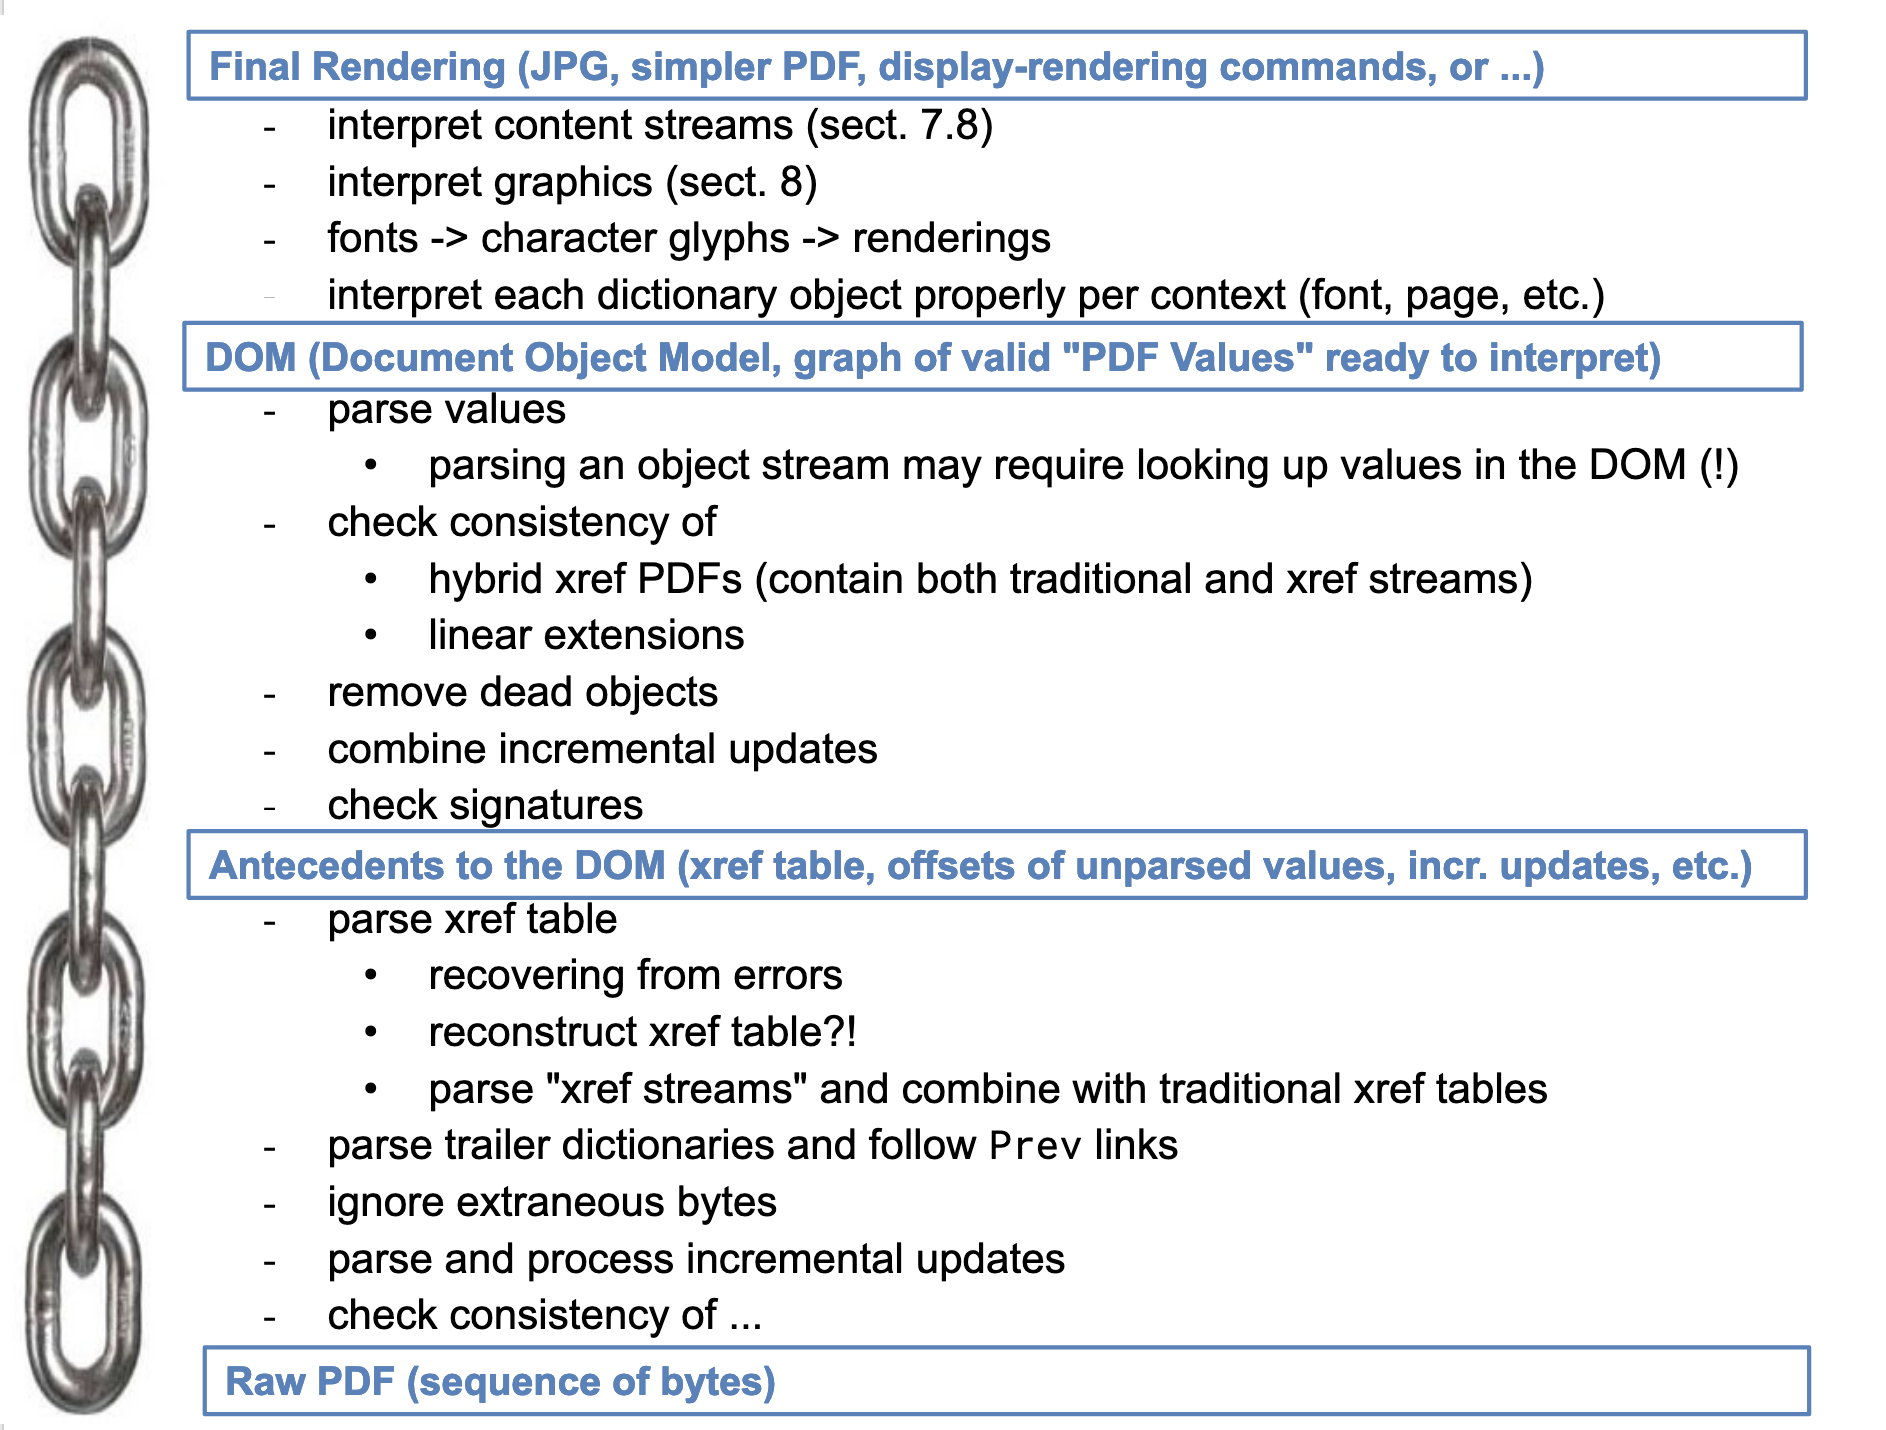
\includegraphics[width=\linewidth]{figures/trustchain-diagram.png}
    \todo{revamp diagram - please add "phase" initiate processing = seek to EOF, locate startxref keyword, etc.}
    \caption{The PDF Trust Chain diagramed.}
    \label{fig:pdf-trust-chain}
\end{figure}

We think understanding a PDF parser in terms of this ``Trust Chain'' is
important:
(1) it highlights the presence of the many ``dependent'' parsers in PDF.
(2) it highlights the importance of ensuring the first/basic/... computations
    (i.e., the pre-DOM parsing and computation) is absolutely secure.
(3) it reminds us that the integrity of the DOM cannot be verified independently
of the lower levels.

% ------------------------------------------------------------------------------
\section{Pre-DOM Vulnerabilities \note{2.5pp}}
\label{sec:predom-vulnerabilities}

\subsection{shadow attacks}
\todo{notion of cavities [belongs?]}

\subsection{schizophrenia arising from ...}
\begin{lstlisting}[style=meta]
  - writer errors
  - parser differentials
    - e.g., ignoring xref tables
  - recovering parsers !!
  - blind faith in incremental updates (Shadow Attacks)
\end{lstlisting}

\subsection{polyglots arising from cavities and permissive implementations and ...}

\subsection{Denial of Service (DOS)}

\begin{lstlisting}[style=meta]
- [potential recursion many places]
- format may not be well-defined because the recursion is not
    "well-defined"
\end{lstlisting}

\subsection{Other?}

% ------------------------------------------------------------------------------
\section{Securing the Pre-DOM Components \note{1pp}}
\label{sec:securing}

There are three major approaches we are taking to improve the security of the
Pre-DOM components of PDF parsing:
\begin{enumerate}
\item
  \emph{Developing tools for inspection and validation of pre-DOM structures.}
  We have developed a tool that ..., this tool validates more of the structure
  than ... .  Using it we can find dead objects and cavities. 
   
\item
  \emph{Writing a formal specification for pre-DOM processing.}
  The PDF specification \cite{pdfspec} is English, not ``formal'', unclear
  in places, \todo{...}

  In \cref{sec:specifying}, we go into much greater detail of our specification.

\item
  \emph{Understanding and clarifying the PDF standard.}
  In the process of doing the above two, we have pushed the bounds
  of our PDF knowledge and have discovered multiple places in which
  \cite{pdfspec} could be made more clear, and also instances in which
  it \todo{...}
  \todo{examples being}
 \item Writing a formal specification (see \cref{sec:specifying}).

 \item Developing Tools
 
 \item Extant data analysis

\end{enumerate}

\todo{the low/first components are most vulnerable...}
     

% ------------------------------------------------------------------------------
\section{Specifying pre-DOM Components \note{4pp}}
\label{sec:specifying}

\subsection{[Motivating Specification]}
\begin{lstlisting}[style=meta]
- [terms: complies with standard, compatible with]
- an implementation
  - should follow the standard
  - should safely support less than standard
  - pragmatically support some common extant data malformations
  - should carefully support more than the standard
  - should not "inf. loop"
    - lots of opportunities - failure to notice digitally signed PDFs that have been tampered! 
      - elaborate?
\end{lstlisting}

\begin{lstlisting}[style=meta]
- Lack of formality in standard. Thus, implementations:
  - are more effort
  - over implement, under implement, wrongly implement
  - backwards and forwards compatibility
  - "backwards parsing"
  - some requirements will not be checked by PDF readers ("writer only" file requirements) 
  - patch existing vs implement from scratch
- No definition of acceptable, reasonable error recovery
- Less than ideal design that reflects 27 years of an evolving standard
- Pre-DOM processing
  - is where many parsing errors & recovery occur
  - is non-trivial
  - involves multiple interdependent features and subtle dialects
  - involves multiple redundant features
    - schizophrenic if these features aren't mutually consistent
\end{lstlisting}

\subsection{The pre-DOM constructs}
\todo{Hmmm: how much detail to go into?
      How will reader understand next section if we say nothing?
}

\subsection{Specifying pre-DOM components}
\begin{lstlisting}[style=meta]
- presented
- going into PDF details, as needed (this section or separate section?)
\end{lstlisting}

% ------------------------------------------------------------------------------
\section{Conclusion \note{1.5pp}}
\label{sec:conclusion}

\subsection{Contributions}

As we discussed in \cref{sec:securing} we have ...
\todo{prosify the following bullet points, split into done/future.}


PDF pre-DOM parsing and semantics:
Clarified aspects of PDF with respect to incremental updates, minor parsing details
Submitted a problem in the definition of cross reference streams (Sec 7.5.8) to
ISO via Peter Wyatt.

Write a proposed implementation/specification for dealing with parsing (DOM-dependent) object streams
Develop formal definitions for pre-DOM parsing/computation

Tool for inspecting and checking PDF at the pre-DOM level:
Created tool for exploring the DOM Antecedent structures as well as validating
them (more than a PDF reader necessarily does).

Based on Galois's \todo{TA2} PDF parser, this tool can
parse and validate each incremental update separately
display "incremental updates," "incremental xref tables," parsed objects, and cavities (bytes that are not used)
validate that object definitions do not overlap (in their source bytes)
      
\subsection{Related Work}

\todo{pdf-hsdriver} 
\todo{Daedalus}
\todo{shadow attacks}
      
\subsection{Future Work}
\todo{...}

Add more features
support linearized files (to improve cavity detection)
more consistency checks: e.g, for hybrid xref files
analysis and categorization of cavities


% ------------------------------------------------------------------------------
\section*{Acknowledgements}

This research was supported by the SafeDocs program under \todo{HR0011-19-C-0073} and HR001119C0079.


\bibliographystyle{plain}
\bibliography{old}
% \bibliography{new}
\todo{Other possible refs: ISO 32000-2:2020, pdf-insecurity.org publications, https://itextpdf.com/en/blog/technical-notes/investigating-pdf-shadow-attacks-depth-pdf-security-using-itext-part-3, K. Koptyra and M. R. Ogiela, “Distributed Steganography in PDF Files - Secrets Hidden in Modified Pages,” Entropy, vol. 22, no. 6, p. 600, May 2020, doi: 10.3390/e22060600.
}

\end{document}
